\section{Vermittlung}

\paragraph{Leitungsvermittlung}
\begin{itemize}
  \item Verbindung ist \emph{durchgehender Kanal} mit konstanter Bandbreite für exklusive Nutzung
  \item \textbf{Multiplexing}: \emph{starres Multiplexing} möglich
  \begin{itemize}
    \item \emph{Frequenzmultiplex}: Feste Zuweisung eines Frequenzabschnitts
    \item \emph{Zeitmultiplex}: Feste Zuweisung eines Zeitschlitz (\emph{time slot}) in jedem Frame
  \end{itemize}
  \item \textbf{Eigenschaften}:
  \begin{itemize}
    \item Aufbau eines durchgehenden Übertragungskanals zwischen Endsystemen
    \item Zwischensysteme: Zustandshaltung statt Adressinformation nötig
    \item zugesicherte, feste Datenrate \( \leadsto \) ungenutzte Ress bei Nichtverwendung
    \item Übertragungsverzögerungen nur physikalisch bedingt \\* \( \leadsto \) keine Schwankungen durch Puffer
    \item Reihenfolgentreue Bitfolgenübertragung
  \end{itemize}
  \item \textbf{Einsatzgebiete}: Telefonnetze, GSM
\end{itemize}

\paragraph{Paketvermittlung}
\begin{itemize}
  \item \textbf{Prinzip}: Weiterleitung anhand von Kontrollinformation in Paket
    (Zieladresse in Datagrammen, lokale Kennung bei virtuellen Verbindungen)
    \item Zwischensysteme Speichern Pakete in \emph{Warteschlangen} \\* \( \leadsto \) Paketverlust möglich, variable Verzögerungszeiten
   \item Üblicherweise Zeitmultiplex (keine Reservierung von Ressourcen)
  \item \textbf{Varianten}:
  \begin{itemize}
    \item \emph{verbindungslos}: Datagramme
    \item \emph{verbindungsorientiert}: virtuelle Verbindungen
  \end{itemize}
\end{itemize}
\begin{figure}[H]\centering\label{Paketvermittlung}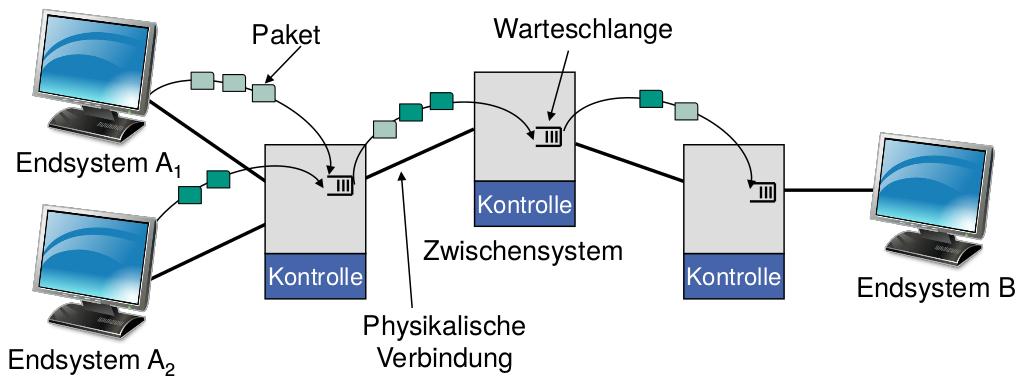
\includegraphics[width=0.33\textwidth]{Paketvermittlung}\end{figure}

\paragraph{Paketvermittlung --- Datagramme}
\begin{itemize}
  \item Pakete (= Datagramme) werden als isolierte Einheiten betrachtet
  \item \textbf{Zieladresse} in jedem Datagramm \( \leadsto \) keine Verbindungsverwaltung nötig
  \item \textbf{Routing}: Pakete können verschiedene Wege im Netz nehmen \\*
    \( \leadsto \) Datagramme können bei Empfänger unsortiert ankommen
\end{itemize}

\paragraph{Paketvermittlung --- virtuelle Verbindungen}
\begin{itemize}
  \item Fester Übertragungsweg zwischen zwei Endsystemen
  \item \textbf{Reihenfolgetreue}: Alle Pakete nehmen den selben Weg
  \item \textbf{Kennung}: \emph{virtual circuit identifier} (VCI) für jeden Übertragungsabschnitt
  \item \textbf{Zieladresse} nur bei Aufbau nötig, Vermittlungsinfo in Zwischensystemen
  \item \textbf{Ablauf}: Verbindungsaufbau \( \to \) Datenübertragung \( \to \) Verbindungsabbau
\end{itemize}

\paragraph{Nachrichtenvermittlung}
\begin{itemize}
  \item \emph{Vermittlung von Anwendungsnachrichten}
  \item Vermittlung üblicherweise mittels mehrerer Pakete
  \begin{itemize}
    \item[\( \leadsto \)] \emph{Segmentierung} und \emph{Reassemblierung} in Zwischensystemen (alle Teile müssen jeweils an gleiches System weitergeleitet werden)
    \item[\( \leadsto \)] \emph{Ende-zu-Ende-Verzögerung wesentlich höher als bei Paketvermittlung}
  \end{itemize}
\end{itemize}

\paragraph{Vermittlungsschicht --- Überblick}
\begin{itemize}
  \item \textbf{Ende-zu-Ende}: transportiert Segmente zwischen Endsystemen
  \item Sender: Kapselt Segmente in Datagramme
  \item Empfänger: Segmente werden an Transportschicht ausgeliefert
  \item Protokolle in \emph{allen} Endsystemen und Routern
  \item \textbf{Router} werten Felder im Kopf aller Datagramme aus, die sie passieren
\end{itemize}

\paragraph{Forwarding und Routing}
\begin{itemize}
  \item \textbf{Forwarding} (\emph{Weiterleitung}): Datenebene
  \begin{itemize}
    \item Pakete werden von Eingang an passenden Ausgang (Tabelle) weitergeleitet
    \item Funktionen lokal in Router
  \end{itemize}
  \item \textbf{Routing} (\emph{Wegewahl}): Kontrollebene
  \begin{itemize}
    \item Ermittelt Wege für Pakete und darauf basierend Weiterleitungstabelle
    \item Betrachtet gesamtes Netz, benötigt Routingalgorithmus und -protokoll
  \end{itemize}
  \item \textbf{Konzepte}:
  \begin{itemize}
    \item traditionell: in jedem Router implementiert, interagieren auf Kontrollebene
    \item \emph{software defined networking} (SDN): in log zentralen Servern implementiert
  \end{itemize}
\end{itemize}

\paragraph{Vermittlungsschicht --- Begriffe}
\begin{itemize}
  \item \textbf{Router}: Auf Vermittlungsschicht operierendes Zwischensystem
  \begin{itemize}
    \item leitet Datagramme mithilfe von Weiterleitungstabelle weiter
    \item tauscht über Routingprotokolle Informationen mit anderen Routern aus
  \end{itemize}
  \item \textbf{Route}: Weg eines Datagramms: Sequenz von Routern zwischen zwei Endsystemen
  \item \textbf{Link}: Übertragungsabschnitt zwischen 2 Routern (kann z.B. auch Brücken enthalten)
  \item \textbf{Port}: Eingangs-/Ausgangs-Netzwerkschnittstelle
\end{itemize}

\paragraph{Vermittlungsschicht --- Protokolle}
\begin{itemize}
  \item \textbf{IP} (\emph{internet protocol}): unzuverlässige Datagrammübertragung
  \item \textbf{ICMP} (\emph{internet control message protocol}): Kontrollinformationsaustausch innerhalb der Vermittlungsschicht
  \item \textbf{ARP} (\emph{address resolution protocol}): Zuordnung von IP-Adressen zu Adressen der Sicherungsschicht
  \item \textbf{RARP} \emph{reverse ARP}: Umkehrfunktionen von ARP
  \item \textbf{BGP} (\emph{border gateway protocol}), \textbf{RIP} (\emph{routing information protocol}), \textbf{OSPF} (\emph{open shortest path first}): Routingprotokolle
\end{itemize}

\paragraph{Vermittlung --- IP (Internet Protocol)}
\begin{itemize}
	\item Verbindungsloser, unzuverlässiger Vermittlungsdienst (kein Kontext in Zwischen- oder Endsystemen)
  \item IP macht die ganze Vermittlung \( \leadsto \) nur ein einziges Vermittlungsprotokoll
  \begin{itemize}
    \item Interoperabilität erhöhen: Anzahl unterschiedlicher Interfaces verringern
    \item Kleinster gemeinsamer Nenner: Anzahl nutzbarer Netze maximieren
  \end{itemize}
\end{itemize}
\begin{figure}[H]\centering\label{IP}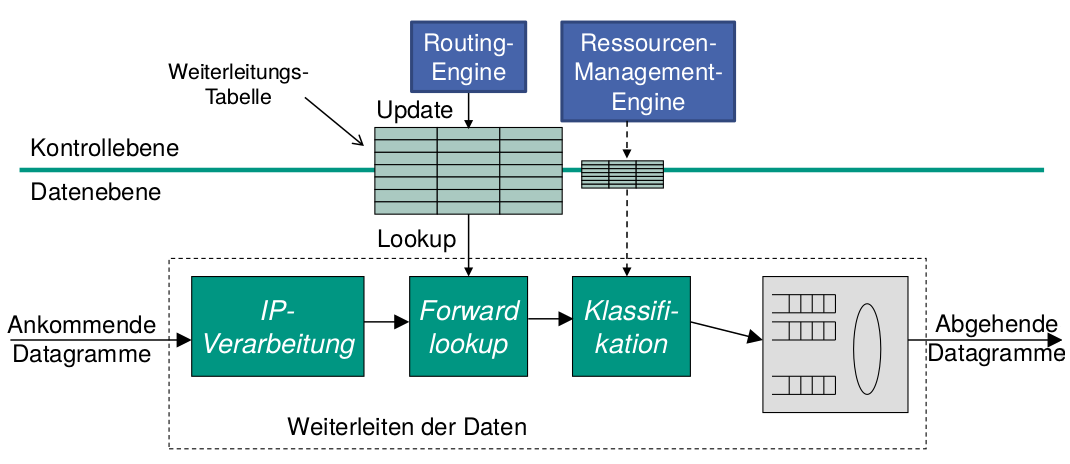
\includegraphics[width=0.4\textwidth]{IP}\end{figure}
\begin{figure}[H]\centering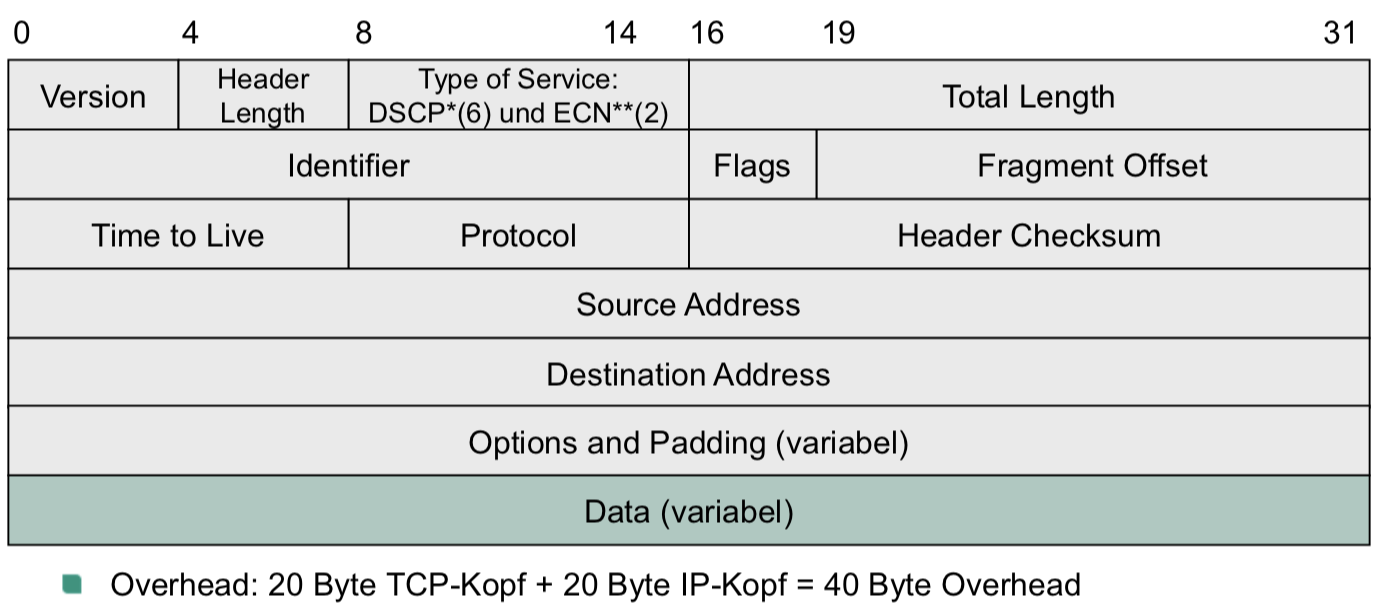
\includegraphics[width=0.4\textwidth]{IP4Header}\end{figure}

\paragraph{IP --- Fragementieren + Reassemblieren}
\begin{itemize}
  \item Anpassung an Maximallänge unterl Netze (\textbf{MTU}: \emph{maximum transfer unit})
  \item Fragmentieren überall möglich, Reassemblieren nur in Endsystem
  \item \textbf{Fragment-Offset} (Einheit: 8 Bytes) + Flag-Felder im IP-Kopf %\\*
\end{itemize}

\paragraph{IP --- Weiterleitung}
\begin{itemize}
  \item \textbf{Endsystem}:
  \begin{itemize}
    \item Rechner mit Zieladresse direkt verbunden \( \to \) Datagramm direkt zustellen
    \item Sonst: Datagramm-Übergabe an Standardrouter
  \end{itemize}
  \item \textbf{Weiterleitungstabelle}: Für jede Zieladresse (Endsystem- oder Netzadresse)
  \begin{itemize}
    \item \emph{Next-Hop-Router} (falls nicht im gleichen Netz)
    \item \emph{Netzschnittstelle}, an die Paket weitergeleitet wird (Schnittstelle, an der Next-Hop bzw. Endsystem hängt)
    \item Flags
  \end{itemize}
\end{itemize}

\paragraph{IP --- Empfangsprozess}
\begin{itemize}
  \item \textbf{Überprüfungen}:
  \begin{itemize}
    \item \emph{Kopflänge}, \emph{Datagrammlänge}, \emph{Prüfsumme}
    \item \emph{Versionsnummer} IP, \emph{Protokoll-Identifikation}
    \item \emph{Lebenszeit}, \emph{Adressklassen}
  \end{itemize}
  \item \textbf{Fehlerfall}: Benachrichtigung ICMP (\emph{internet control message protocol}) --- möglicherweise wird ICMP-Paket ausgesendet
\end{itemize}

\paragraph{IP --- Adressierung}
\begin{itemize}
  \item \textbf{Ziel}: Eindeutige Identifizierung aller Interfaces von Routern/Endsystemen
  \item \textbf{IP-Adressen}: Adressen der Vermittlungsschicht -- Kennung für Interfaces
  \begin{itemize}
    \item \emph{IPv4}: 32 Bit (z.B. 207.142.131.235)
    \item \emph{IPv6}: 128 Bit (z.B. 2001:0db8:85a3:08d3:1319:8a2e:0370:7344)
  \end{itemize}
  \item IP-Adresse unterteilt in
  \begin{itemize}
    \item \emph{Subnetz-Teil}: high order bits
    \item \emph{Endsystem-Teil}: low order bits
  \end{itemize}
  \item \textbf{Subnetz}: Interfaces mit selbem Subnetz können ohne Router kommunizieren
  \item \textbf{CIDR} (Classless Inter-Domain Routing): Subnetz-Teil kann unterschiedlich lang sein (Format: a.b.c.d/x, x = Anzahl Bits im Subnetz-Teil, z.B. 200.23.16.0/24)
  	
\end{itemize}

\paragraph{Adresszuteilung}
\begin{itemize}
	\item \textbf{Provider}: Erhält Block von \textbf{ICANN} (\emph{internet corporation for assigned names/numbers}), allokiert IPs, verwaltet DNS, weist Domainnamen zu
	\item Netz bekommt Subnetz-Teil von seinem Provider zugeordnet
  \item \textbf{Manuell}: Durch Systemadministrator
  \item \textbf{Dynamisch}: DHCP-Server liefert auf Anfrage IP-Adresse für Client
\end{itemize}

\paragraph{DHCP (dynamic host configuration protocol)}
\begin{itemize}
	\item Dynamischer Bezug von IP-Adressen durch Endsysteme
	\item Beschränkte zeitliche Gültigkeit (\emph{lease})
	\item Zusätzlich Subnetzmaske, Adresse Default-Gateway, DNS-Server, \dots möglich
	\item \textbf{Ablauf}: [Discover, Offer], Request, Ack (jeweils als Broadcast)
\end{itemize}

\paragraph{Internet Control Message Protocol (ICMP)}
\begin{itemize}
  \item Einzelne Datagrammverluste meldet IP nicht (unzuverlässiger Dienst)
  \item Schwerwiegende Probleme (z.B. Leitungsunterbrechung): Mitteilung via ICMP
  \item[\( \Rightarrow \)] ICMP tauscht Fehlernachrichten, Statusanfragen, Zustandsinfos aus
  \item \textbf{Echo} + Antwort (\emph{echo and echo reply}):
  \begin{itemize}
    \item Aktivitätsüberprüfung von Kommunikationssystemen
    \item Empfänger Echo-Anfrage sendet erhaltene Daten in Echo-Antwort zurück
  \end{itemize}
  \item \textbf{Zeitstempel} + Antwort (\emph{timestamp and timestamp reply}): Bestimmung von Umlaufzeiten (\emph{round trip time}, RTT)
\end{itemize}

\paragraph{IPv6}
\begin{itemize}
  \item \textbf{Problem}: Adressraum IPv4 geht aus \( \Rightarrow \) Erhöhung Adresslänge 32 auf 128 Bit 
  \item Optimiere \textbf{Format des Headers} für schnelle Verarbeitung:
  \begin{itemize}
    \item feste Kopflänge (40 Byte), Optionen als Erweiterungsköpfe (\emph{next header})
    \item keine Unterstützung von Fragmentierung, keine Prüfsumme
  \end{itemize}
   \item ICMPv6: neue Version von ICMP
    \begin{figure}[H]\centering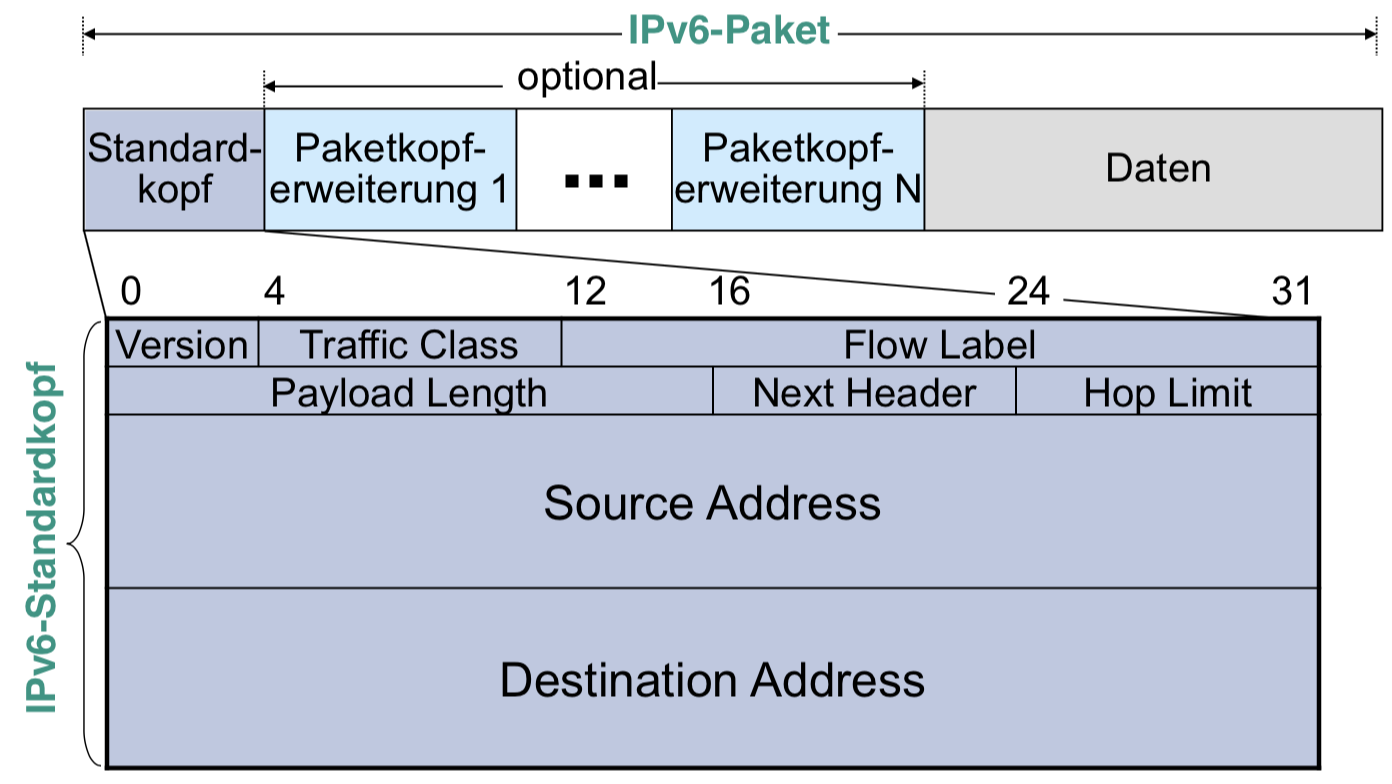
\includegraphics[width=.7\linewidth]{IP6Header}\end{figure}
\end{itemize}

\paragraph{Routing --- Prinzipien}
\begin{itemize}
  \item \textbf{Ziel}: Guten Weg durch Netz finden (geringste Kosten)
  \item \textbf{Netzgraph}: Netz wird als Graph verstanden
  \begin{itemize}
    \item \emph{Knoten}: Router
    \item \emph{Kanten}: Übertragungsabschnitte (Kantenkosten z.B. Verzögerung, Preis,\dots)
  \end{itemize}
  \item \textbf{Pfad}: Folge von Knoten (meist Pfad mit kürzester Länge gesucht)
\end{itemize}

\paragraph{Routing-Verfahren --- Dynamik}
\begin{itemize}
  \item \textbf{Nicht adaptiv}: Routen ändern sich selten, wesentlich seltener als Verkehr
  \item \textbf{Adaptiv}: Routen ändern sich abhängig von Verkehr und Topologie
  \begin{itemize}
    \item Routenänderungen periodisch oder reaktiv
    \item \emph{Zielkonflikt}: Systeme haben ggf kein Live-Abbild des Netzes, ggf hohe Netzbelastung durch Routing-Informationsaustausch
  \end{itemize}
\end{itemize}

\paragraph{Routing-Verfahren --- statisches Routing}
\textbf{Beispiel}: Abhängig von Zufallszahl weiterleiten nach B, C oder D

\paragraph{Routing-Verfahren --- zentralisiert}
\begin{itemize}
  \item Adaptives Verfahren
  \item \textbf{Routing Control Center}: Für Berechnung/Verteilung der optimalen Pfade \\* \( \to \) Systeme senden periodisch Zustand an RCC (aktive Nachbarn, Warteschlangenlängen,\dots)
  \item \textbf{Vorteile}:
  \begin{itemize}
    \item RCC hat alle Informationen \( \leadsto \) kann perfekte Entscheidungen treffen
    \item Systeme müssen kein Routing betreiben
  \end{itemize}
  \item \textbf{Nachteile}:
  \begin{itemize}
    \item Berechnungsdauer für große Netze ggf sehr lang
    \item Ausfall RCC lähmt ganzes Netz
    \item Inkonsistenzen möglich, da RCC-nahe Systeme Tabellen schneller erhalten
    \item starke Belastung des RCC
  \end{itemize}
\end{itemize}

\paragraph{Routing-Verfahren --- isoliert}
\begin{itemize}
  \item \textbf{Prinzip}: Jedes System entscheidet nur anhand eigener Informationen
  \item kein Austausch von Routinginformationen zwischen Systemen
  \item \textbf{Fluten}: Jedes eingehende Datagramm auf jeder Übertragungsleitung weiterleiten
  \item \emph{Fluteindämmung}:
  \begin{itemize}
    \item \emph{Sequenznummern} für Duplikaterkennung
    \item \emph{Lebensdauerkontrolle} durch Zählen der Übertragungsabschnitte (\emph{hops})
  \end{itemize}
  \item \emph{Varianten}:
  \begin{itemize}
    \item \emph{selektives Fluten}: Weiterleitung nicht auf allen Übertragungsabschnitten
    \item \emph{random walk}: Zufällige Auswahl eines Übertragungsabschnittes
  \end{itemize}
  \item \textbf{Hot Potato}: Datagramme so schnell wie möglich weiterleiten \\*
    \( \leadsto \) Übertragungsabschnitt mit kürzester Warteschlange wählen
  \item \emph{Varianten}:
  \begin{itemize}
    \item nie an Herkunftsleitung weiterleiten
    \item Kombination mit statischem Routing: statisches Verfahren zur Auswahl von Leitung mit Warteschlangenlänge unter Schwellwert
  \end{itemize}
\end{itemize}

\paragraph{Routing-Verfahren --- Verteiltes adaptives Routing}
\begin{itemize}
  \item \textbf{Prinzip}: Systeme tauschen Routing-Informationen mit Nachbarn aus, jedes System unterhält Routing-Tabelle
  \item \textbf{Varianten}:
  \begin{itemize}
    \item periodischer Informationsaustausch
    \item Austausch nur bei größeren Änderungen
  \end{itemize}
\end{itemize}

\paragraph{Routing-Algorithmen --- Übersicht}
\begin{itemize}
  \item \textbf{Distanz-Vektor-Algorithmen}:
  \begin{itemize}
    \item Distanz als Routing-Metrik
    \item jeder Router kennt Distanz zu allen anderen Systemen im Netz
    \item dazu Austausch der Distanzen zwischen Nachbarn
    \item \emph{Problem}: kürzerer langsamer Weg wird längerem schnelleren vorgezogen
  \end{itemize}
  \item \textbf{Link-State-Algorithmen}:
  \begin{itemize}
    \item Unterschiedliche Routing-Metriken
    \item berücksichtigt aktuelle Zustände der Netzanschlüsse
    \item jeder Router kennt und nutzt ganze Netztopologie zur Berechnung
  \end{itemize}
\end{itemize}

\paragraph{Link-State vs. Distanz-Vektor}
\begin{itemize}
	\item \textbf{Komplexität Kontroll-Pakete}:
	\begin{itemize}
    \item \emph{Link-State}: jedes System muss Kosten aller Links kennen, Änderungen müssen an alle Systeme geschickt werden \( \leadsto  O(nE) \) Pakete
    \item \emph{Distanz-Vektor}: Änderungen nur an benachbarte Systeme weitergegeben
  \end{itemize}
	\item \textbf{Konvergenzgeschwindigkeit}:
	\begin{itemize}
    \item \emph{Link-State}: schnelle Konvergenz, schleifenfrei, Oszillationen möglich
    \item \emph{Distanz-Vektor}: langsame Konvergenz, Schleifen + Count-to-\( \infty \) möglich
  \end{itemize}
	\item \textbf{Robustheit}:
	\begin{itemize}
    \item \emph{Link-State}: Routenberechnungen separiert \( \leadsto \) Robustheit
    \item \emph{Distanz-Vektor}: ein System kann inkorrekte Pfade zu allen Zielen verbreiten
  \end{itemize}
	\item \textbf{Fazit}:
	\begin{itemize}
    \item \emph{Link-State}: Konvergiert schneller, ist robuster
    \item \emph{Distanz-Vektor}: einfacher zu implementieren
  \end{itemize}
\end{itemize}

\paragraph{Routing-Algorithmen --- Distanz-Vektor}
\begin{itemize}
    \item \textbf{verteilt}: jeder Router erhält Infos von direkten Nachbarn, führt Berechnung durch und verteilt dann neue Informationen an direkte Nachbarn
    \item \textbf{iterativ}: Verteilen + Berechnen von Informationen so lange, bis keine Information mehr ausgetauscht wird

\end{itemize}

\paragraph{Distanz-Vektor --- Distanz-Vektor-Tabelle}
\begin{itemize}
	\item \textbf{Distanz-Vektor-Tabelle}:
	\begin{itemize}
    \item Grundlegende, in jedem System vorhandene Datenstruktur
    \item Zeilen für alle möglichen Ziele, Spalten für direkte Nachbarn
  \end{itemize}
  \item \textbf{Beispiel}: \( X \) will Daten über direkten Nachbar \( Z \) an \( Y \) weiterleiten \\* \( \leadsto D^X(Y,Z) = c(X,Z) + \underset{w}{\text{min}}\{ D^Z(Y,w) \} \)
  \item \textbf{Beispiel}: \( D^E(A,D) \)
  \begin{itemize}
    \item erster Übertragungsabschnitt: \( E \to D \)
    \item Tabelleneintrag: Kosten \( E \to D \) (2) + minimale Kosten \( D \to A \) (3)
  \end{itemize}
\end{itemize}
\begin{figure}[H]\centering\label{DistanzVektor}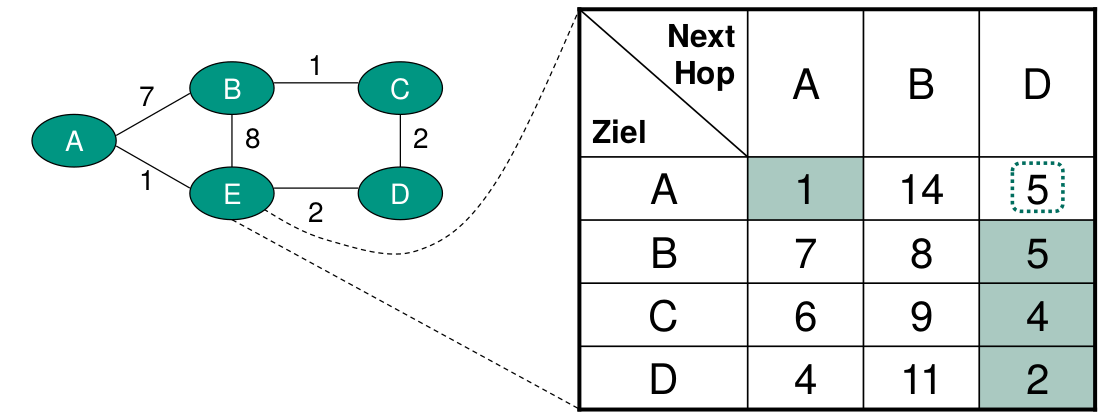
\includegraphics[width=.7\linewidth]{DistanzVektor}\end{figure}

\paragraph{Distanz-Vektor --- Distanz-Vektor-Algorithmus}
\begin{itemize}
  \item von Bellman und Ford
  \item \textbf{Initialisierung}:
  \begin{itemize}
    \item für alle Nachbarn \( v \): \( D^X(*,v) = \infty \), \( D^X(v,v) = c(X,v) \)
    \item für alle Ziele \( y \): sende \( \underset{w}{\text{min}}D^X(y,w) \) allen Nachbarn (\( w \) enthält Nachbarn)
  \end{itemize}
  \item \textbf{Schleife}:
  \begin{itemize}
    \item geänderte Abschnittskosten: für alle Ziele \( y \): \( D^X(y,V) \coloneqq D^X(y,V) + d \)
    \item Update von Nachbarn: kürzester Pfad von \( V \) zu Ziel \( Y \) um \( \alpha \) geändert \\* \( \leadsto \) \( D^X(Y,V) \coloneqq c(X,V) + \alpha \) \\* \( \leadsto \) Falls neuer Minimalwert für ein Ziel \( Y \),  sende an alle direkten Nachbarn
  \end{itemize}
  \item \textbf{Komplexität}: \( O(n^2k) \) für \( n \) Knoten und \( k \) Kanten
\end{itemize}

\paragraph{Distanz-Vektor --- Updateausbreitung}
\begin{itemize}
  \item \textbf{Good news}: schnelle Ausbreitung
  \item \textbf{Bad news}: langsame Ausbreitung, ggf Routing-Schleifen \\*
    \( \leadsto \) \textbf{Count to Infinity-Problem}
  \item \textbf{Poisoned Reverse}: Vermeidung von Routing-Schleifen, indem Routing-Information \( Y \) vorenthalten wird, wenn Weg über \( Y \) kürzer
\end{itemize}

\paragraph{Routing-Algorithmen --- Link-State-Routing}
\begin{itemize}
  \item \textbf{Prinzip}: Jedes System berechnet kürzeste Pfade durch gesamtes Netz
  \begin{itemize}
    \item Systeme müssen zu Beginn nur direkte Nachbarn kennen
    \item Entdecken von neuen Nachbarn zB mittels \code{HELLO}-Pakete
    \item \emph{link state broadcast}: Identität + Kosten zu Nachbarn werden allen Routern im Netz weitergeleitet (Fluten)
    \item Systeme lernen Topologie durch LSBs der anderen Systeme
    \item \emph{Ergebnis}: Alle Systeme haben \emph{identisches} Wissen über Netz
  \end{itemize}
  \item \textbf{Implementierung}: Dijkstra-Algorithmus
\end{itemize}

\paragraph{software defined networking}
\begin{itemize}
  \item \textbf{Zentrale Eigenschaften}:
  \begin{itemize}
    \item Separierung von Kontroll- und Datenebene
    \item Flow-basierte Paketweiterleitung
    \item Logik an externen Controller ausgelagert
    \item Netzwerk programmierbar
  \end{itemize}
  \item \textbf{Umsetzung}: \emph{open flow}-Protokoll (quasi-Standard, Alternativen existieren) \\* \( \to \) regelt Kommunikation zwischen Controller und Switch
\end{itemize}

\paragraph{Traditionelles IP-Routing}
\begin{itemize}
  \item Kontroll- und Datenebene in jedem Router
  \item \textbf{Vorteile}:
  \begin{itemize}
    \item Ausfallsicherheit (selbstorganisiert, verteilte Kontrolle, hohe Redundanz)
    \item Schnelle Reaktion (optim Routing-Hardware, lokale Routingentscheidung)
    \item Bewährtes Konzept
  \end{itemize}
  \item \textbf{Nachteile}:
  \begin{itemize}
    \item proprietäre Management-Schnittstellen (Mischbetrieb schwierig)
    \item unflexibel (neue Funktionen hzfg schwierig, aufwändige Standardisierung)
    \item teuer (hochqualifiziertes Personal + Overprovisioning benötigt)
  \end{itemize}
\end{itemize}

\paragraph{SDN-Routing}
\begin{itemize}
  \item \textbf{Vorteile}:
  \begin{itemize}
    \item logisch zentralisierte Sicht (Controller hat Netzüberblick, einfacher Einsatz von Graphenalgorithmen)
    \item neue Funktionalität in Software (als App im Controller, kürzere Entwicklungszeit)
    \item Trennung von Kontroll- und Datenebene (Innovationen unabhängig möglich, herstellerunabhängig durch offene Schnittstellen)
  \end{itemize}
  \item \textbf{Nachteile}:
  \begin{itemize}
    \item Skalierbarkeit
    \item \emph{single point of failure}
    \item Kommunikation mit Controller langsam
  \end{itemize}
\end{itemize}
\begin{figure}[H]\centering\label{SDNRouting}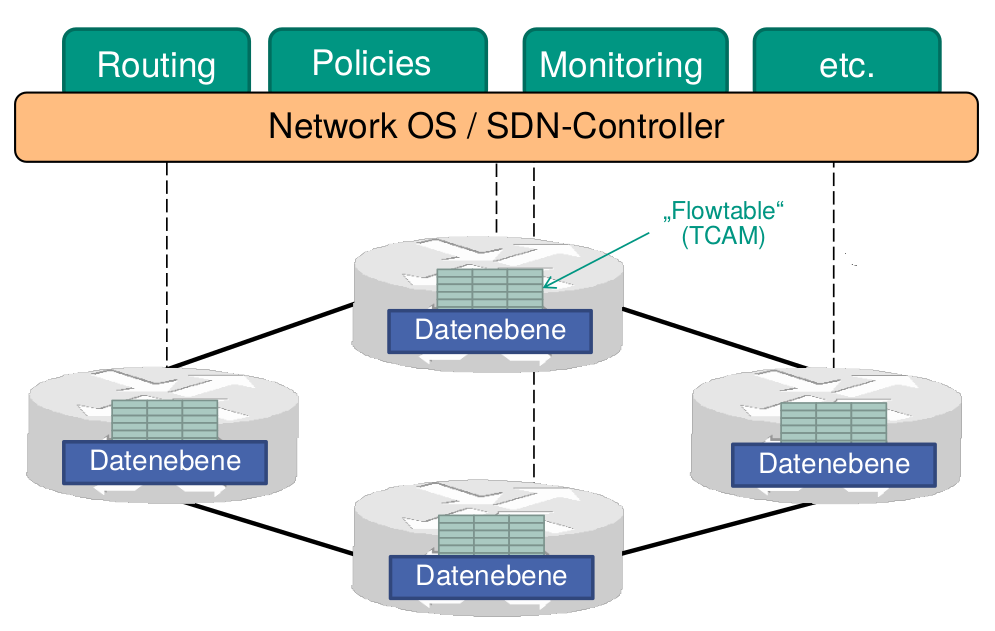
\includegraphics[width=.5\linewidth]{SDNRouting}\end{figure}

\paragraph{SDN --- Paketweiterleitung}
\begin{itemize}
  \item \textbf{Traditioneller IP-Router}: kennt keine Flows, Weiterleitung über Ziel-IP-Adresse (Longest Prefix Matching)
  \item \textbf{SDN-Switch}: Weiterleitung über Flowtable, nutzt verschiedene IP-Kopf-Felder, speichert Zustand pro Flow
\end{itemize}
\begin{figure}[H]\centering\label{SDNFlow}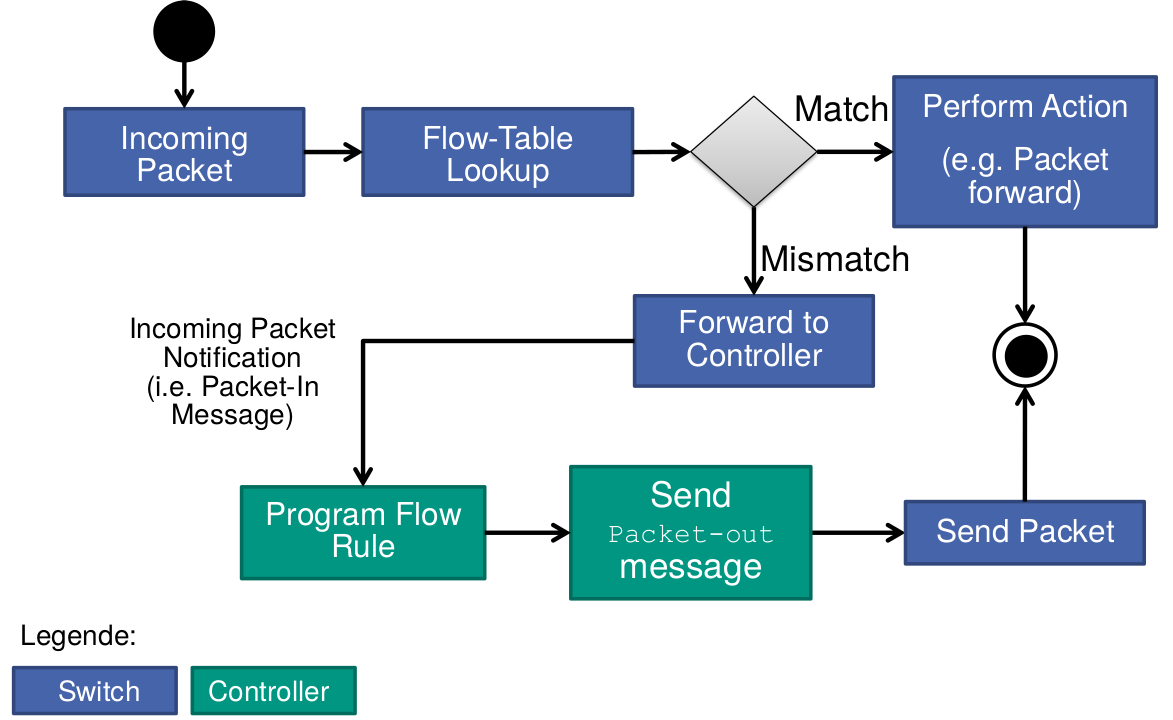
\includegraphics[width=.8\linewidth]{SDNFlow}\end{figure}